%%%%%%%%%%%%%%%%%%%%%%%%%%%%%%%%%%%%%%%%%%%%%%%%%%%%%%%%%%%%%%%%%%%%%%%%%%%%%%%%%%%%%%%%%%%%%%%%%%%%%%%
%%														%%
%% 				DIPLOMOVÁ PRÁCE - Tomáš Klemsa			%%
%% 				 										%%
%%														%%
%% pro formátování využita šablona: http://geo3.fsv.cvut.cz/kurzy/mod/resource/view.php?id=775 	%%
%%													%%
%%%%%%%%%%%%%%%%%%%%%%%%%%%%%%%%%%%%%%%%%%%%%%%%%%%%%%%%%%%%%%%%%%%%%%%%%%%%%%%%%%%%%%%%%%%%%%%%%%%%%%% 

\documentclass[%
  12pt,         			% Velikost základního písma je 12 bodů
  a4paper,      			% Formát papíru je A4
  oneside,       			% Oboustranný tisk
  pdftex,				    % překlad bude proveden programem 'pdftex' do PDF
%%%  draft
]{report}       			% Dokument třídy 'zpráva'
%

\newcommand{\Fbox}[1]{\fbox{\strut#1}}

% Code
\usepackage{minted}


\usepackage[czech, english]{babel}	% použití češtiny, angličtiny
\usepackage[utf8]{inputenc}		% Kódování zdrojových souborů je UTF8

\usepackage[square,sort,comma,numbers]{natbib}

\usepackage{caption}
\usepackage{subcaption}
\captionsetup{font=small}
\usepackage{enumitem} 
\setlist{leftmargin=*} % bez odsazení

\makeatletter
\setlength{\@fptop}{0pt}
\setlength{\@fpbot}{0pt plus 1fil}
\makeatletter

\usepackage[dvips]{graphicx}   
\usepackage{color}
\usepackage{transparent}
\usepackage{wrapfig}
\usepackage{float} 

\usepackage{cmap}           
\usepackage[T1]{fontenc}    

\usepackage{textcomp}
\usepackage[compact]{titlesec}
\usepackage{amsmath}
\addtolength{\jot}{1em} 

\usepackage{chngcntr}
\counterwithout{footnote}{chapter}

\usepackage{acronym}

\usepackage[
    unicode,                
    breaklinks=true,        
    hypertexnames=false,
    colorlinks=true, % true for print version
    citecolor=black,
    filecolor=black,
    linkcolor=black,
    urlcolor=black
]{hyperref}         

\usepackage{url}
\usepackage{fancyhdr}
%\usepackage{algorithmic}
\usepackage{algorithm}
\usepackage{algcompatible}
\renewcommand{\ALG@name}{Pseudokód}% Update algorithm name
\def\ALG@name{Pseudokód}

\usepackage[
  cvutstyle,          
  diploma        
]{thesiscvut}


\newif\ifweb
\ifx\ifHtml\undefined % Mimo HTML.
    \webfalse
\else % V HTML.
    \webtrue
\fi 

\renewcommand{\figurename}{Obrázek}
\def\figurename{Obrázek}

%%%%%%%%%%%%%%%%%%%%%%%%%%%%%%%%%%%%%%%%%%%%%%%%%%%%%%%%%%%%%%%%%
%%%%%%%%%%% Definice informací o dokumentu  %%%%%%%%%%%%%%%%%%%%%
%%%%%%%%%%%%%%%%%%%%%%%%%%%%%%%%%%%%%%%%%%%%%%%%%%%%%%%%%%%%%%%%%

%% Název práce
\nazev{Název}
{Title}

%% Jméno a příjmení autora
\autor{Tomáš}{Klemsa}

%% Jméno a příjmení vedoucího práce včetně titulů
\garant{Jméno vedoucího}

%% Označení oboru studia
\oborstudia{Geomatika}{}

%% Označení ústavu
\ustav{Katedra geomatiky}{}

%% Rok obhajoby
\rok{2020}

%Mesic obhajoby
\mesic{červen}

%% Místo obhajoby
\misto{Praha}

%% Abstrakt
\abstrakt 
{ 	\parindent=1cm Abstrakt....................................... }
{	\parindent=1cm Abstract.......................................  }

%% Klíčová slova
\klicovaslova
{klíčová slova}
{Key worlds}

%%%%%%%%%%%%%%%%%%%%%%%%%%%%%%%%%%%%%%%%%%%%%%%%%%%%%%%%%%%%%%%%%%%%%%%%

%%%%%%%%%%%%%%%%%%%%%%%%%%%%%%%%%%%%%%%%%%%%%%%%%%%%%%%%%%%%%%%%%%%%%%%%
%% Nastavení polí ve Vlastnostech dokumentu PDF
%%%%%%%%%%%%%%%%%%%%%%%%%%%%%%%%%%%%%%%%%%%%%%%%%%%%%%%%%%%%%%%%%%%%%%%%
\nastavenipdf
%%%%%%%%%%%%%%%%%%%%%%%%%%%%%%%%%%%%%%%%%%%%%%%%%%%%%%%%%%%%%%%%%%%%%%%

%%% Začátek dokumentu
\begin{document}

\catcode`\-=12  % pro vypnuti aktivniho znaku '-' pouzivaneho napr. v \cline 

% aktivace záhlaví
\zahlavi

% předefinování vzhledu záhlaví
\renewcommand{\chaptermark}[1]{%
	\markboth{\MakeUppercase
	{%
	\thechapter.%
	\ #1}}{}}

% Vysázení přebalu práce
%\vytvorobalku

% Vysázení titulní stránky práce
\vytvortitulku

% Vysázení listu zadani
\stranka{}%
	%{\includegraphics[scale=0.7]{./zadani.jpg}}%\sffamily\Huge\centering\ }%ZDE VLOŽIT LIST ZADÁNÍ}%
	%{\sffamily\centering Z~důvodu správného číslování stránek}

% Vysázení stránky s abstraktem
\vytvorabstrakt

% Vysázení prohlaseni o samostatnosti
\vytvorprohlaseni

% Vysázení poděkování
\stranka{%nahore
       }{%uprostred
       }{%dole
       \sffamily
	\begin{flushleft}
		\large
		\MakeUppercase{Poděkování}
	\end{flushleft}
	\vspace{1em}
		%\noindent
	\par\hspace{2ex}
	{Poděkování...}
}


% Vysázení obsahu
\obsah

% Vysázení seznamu tabulek
%\seznamtabulek

% jednotlivé kapitoly
\chapter{Úvod}
	Fotogrammetrie je obor zabývající se geometrickými vztahy mezi objekty zachycenými na fotografickém snímku. Tento způsob se často využívá u dokumentace historických objektů, tvorby map z leteckých snímků, při dokumentaci dopravních nehod atd. Fotogrammetrii můžeme rozdělit do více kategorií.
	
	\textbf{Jednosnímková fotogrammetrie}
	
	Nejjednodušší metoda je tzv. jednosnímková fotogrammetrie. Jak název napovídá, je zpracováván pouze jeden snímek. Metoda je hojně využívána u dokumentace fasád budov. Omezení při tomto postupu je, že ze snímku získáme pouze dvojrozměrnou informaci, proto jakákoliv hloubková členění budou oproti zvolené rovině zkreslená.
	
	\textbf{Stereofotogrammetrie}
	
	Metoda využívající stereoskopického vjemu, na jehož základě získáme z dvou překrývajících se snímků s rovnoběžnou osou záběru prostorové informace. Tato metoda je hojně využívána v letecké fotogrammetrii.

	\textbf{Průseková fotogrammetrie}
	
	Průseková fotogrammetrie využívá více snímků s nerovnoběžnou osou záběru, na kterých jsou vyhledány identické body, ze kterých jsou získané prostorové souřadnice těchto bodů.
	
	\textbf{Obrazová korelace}
	
	
	Obrazová korelace, hojně nazývána také jako IBMR (\textit{Image Based Modeling and Rendering}) je metoda využívající obrazovou korelaci pro vyhledávání identických bodů. Funguje v podstatě na principu průsekové fotogrammetrie s tím rozdílem, že je potřeba velké množství snímků a algoritmus SIFT (\textit{Scale Invariant Feature Transformation}), který vyhledává identické body, proto je vhodná pro objekty negeometrického tvaru.
	
	Všechny tyto metody využívají obrazová data, u kterých je předpoklad středového promítání. To ovšem u fotoaparátů s běžným objektivem neplatí. Fotografie jsou zatíženy geometrickým zkreslením, které by se projevilo na kvalitě výstupu. Proto je nutné toto zkreslení redukovat.

	Tato bakalářská práce je zaměřena na tvorbu jednoduchého a uživatelsky přívětivého softwaru pro odstranění geometrického zkreslení fotografických snímků na základě znalosti prvků vnitřní orientace včetně průběhu radiální a tangenciální distorze. Průběh distorze může být vyjádřen různými způsoby. Pro tvořený program byl však zvolen model podle Duane C. Browna, který je často využívaným modelem ve fotogrammetrických softwarech.
	
	Existuje mnoho programů, které umí nežádoucí zkreslení ze snímků odstranit. Proč tedy vyvíjet nástroj nový? 
	
	Jako první bych zmínil grafické editory. Jedná se o nástroje, které většinou umí odstranit zkreslení na základě subjektivního vnímání uživatele. Například tak, že posuvníkem uživatel nastavuje velikost zkreslení, až stěny budovy nejsou prohnuté. Tyto nástroje jsou ovšem vhodné pouze pro fotografie, které nebudou fotogrammetricky zpracovávány. Nepracují totiž s tangenciální distorzí, souřadnicemi hlavního snímkového bodu a nastavení průběhu radiální distorze je často velmi omezené. 
	
	Do druhé skupiny bych zařadil programy fotogrammetrické. Často profesionální a velmi obsáhlý software, který je ovšem v mnohých případech finančně nákladný. V některých případech tyto programy mají funkci na poloautomatický výpočet prvků vnitřní orientace, což je značná úspora času.\par


\section{Cíle práce}
	Cílem této práce je tedy vytvořit program, který bude volně šiřitelný, aby kdokoliv měl možnost upravovat, šířit a dále využívat zdrojový kód a bude psán v rozšířeném multiplatformním objektově orientovaném programovacím jazyce, tak aby byla snadná jeho další úprava. Program byl tedy vytvořen v jazyce \textit{C++} na platformě \textit{Qt}.


\chapter{Rešerše používaných algoritmů}
Tato kapitola se zabývá přehledem používaných algoritmů pro výpočet polygonů ze vstupních linií. Polygonizace, v případě výskytu fuzzy průsečíků, se zpravidla neřeší jedním algoritmem na polygonizaci, ovšem průsečíky linií jsou nejprve doplněny a poté se zahájí vlastní tvorba polygonů z těchto upravených linií. Toto řešení používají i v praxi užívané GIS nástroje, jako například nástroj \textit{"Polygonize"} využívaný v softwaru \textit{QGis}, nebo nástroj \textit{"Feature To Polygon"} ze softwaru \textit{ArcGIS}.

\textbf{TODO: tady by bylo fajn citovat buďto dokumentaci QGis nebo vlastní repozitář... u arcgis je toto tvrzení založeno jen na výstupu aplikace v task history.}

\section{Výpočet průsečíků množiny linií}
Výpočet všech průsečíků množin linií lze provést snadno, testováním všech úseček se všemi. Tímto postupem ovšem zjevně dosáhneme složitosti $\mathcal{O}(N^2)$. Pro výpočet průsečíků lze ovšem využít i algoritmus s časovou náročnosti $\mathcal{O}(n\log{}n)$, známý také jako Bentley–Ottmannův algoritmus \cite{bentley1979algorithms}.

\subsection{Vzájemná poloha dvou úseček}
Ve 2D výpočetní geometrii jsou standardně jednotlivé segmenty linie vyjádřeny počátečním a koncovým bodem. Uvažujme tedy že máme dány 2 přímky $p_1 = |S_1 E_1|$ a $p_2 = |S_2 E_2|$, kde $S_1 = [x_{S1},y_{S1}]$, $E_1 = [x_{E1},y_{E1}]$, $S_2 = [x_{S2},y_{S2}]$, $E_2 = [x_{E2},y_{E2}]$ a potřebujeme provést test, zda se dané přímky protínají či nikoliv, můžeme použít takzvaný \textit{Half-Plane} test, tedy test, který určuje zda bod leží v pravé či levé polorovině od přímky. Tento test zopakujeme celkem čtyřikrát a to na počáteční a koncový bod druhé úsečky, abysme zjistili zda se přímky protínají. Test je založen na výpočtu orientace dvou vektorů $\vec{u}$  a $\vec{v}$, kde vektor $\vec{v}$ je směrový vektor úsečky, tedy $\overrightarrow{S_1E_1}$ a vektor $\vec{v}$ je vektor $\overrightarrow{S_1S_2}$.

	

	

\begin{figure}[h]
  \centering
  \includegraphics[width=12cm]{./pictures/2/half-plane_vector.pdf}
  \caption{\textit{Half-plane} test}
  \label{fig:2-half_plane_vector}
\end{figure}

\begin{figure}[h]
    \centering % <-- added
\begin{subfigure}{0.5\textwidth}
  \includegraphics[width=\linewidth]{./pictures/2/half-plane_1.pdf}
  \caption{Test bodu $S_2$ k přímce $|S_1E_1|$}
  \label{fig:2-half_plane_1}
\end{subfigure}\hfil % <-- added
\begin{subfigure}{0.5\textwidth}
  \includegraphics[width=\linewidth]{./pictures/2/half-plane_2.pdf}
  \caption{Test bodu $E_2$ k přímce $|S_1E_1|$}
  \label{fig:2-half_plane_2}
\end{subfigure}\hfil % <-- added

\medskip
\begin{subfigure}{0.5\textwidth}
  \includegraphics[width=\linewidth]{./pictures/2/half-plane_3.pdf}
  \caption{Test bodu $S_1$ k přímce $|S_2E_2|$}
  \label{fig:2-half_plane_3}
\end{subfigure}\hfil % <-- added
\begin{subfigure}{0.5\textwidth}
  \includegraphics[width=\linewidth]{./pictures/2/half-plane_4.pdf}
  \caption{Test bodu $E_1$ k přímce $|S_2E_2|$}
  \label{fig:2-half_plane_4}
\end{subfigure}\hfil % <-- added
\caption{Grafické znázornění \textit{Half-plane} testů pro zjištění existence průsečíku}
\label{fig:2-half_plane}
\end{figure}

\subsection{Bentley–Ottmannův algoritmus}
Tento algoritmus je založen na technice zvané \textit{sweep line}, překládané jako \textit{zametací přímka}, pro kterou je předpokladem mít setříděná vstupní data, podle jedné ze souřadnic. Algoritmus zde nebuda více popisován jelikož je velmi dobře vysvětlen v těchto publikacích \cite{bentley1979algorithms} \cite{bayer2008algoritmy}.

\section{Polygonizace}
Jak již bylo řečeno, polygonizace se provádí nad daty s doplněnými průsečíky linií. Doplnění průsečíku jsme schopni vyřešit v čase $\mathcal{O}(n\log{}n)$. Nyní tedy nastává otázka jak řešit vlastní polygonizaci.


\section{GIS software}
Provedení polygonizace zvládá většina současně používaného GIS softwaru. Pokusíme se tedy rozebrat postupy jednotlivých nástrojů na polygonizaci.

\subsection{ArcGIS}
ArcGIS je vyvíjený společností Esri, v současné době se jedná o nejpokročilejší nástroj v oblasti GIS. Jedná se o proprietární software, u kterého 


\subsection{QGis}
QGis je nejspíše jeden z nejznámějších volných nástrojů pro práci v GIS. Je šířen pod copyleftovou  licencí \textit{GNU General Public License}, tudíž máme volný přístup ke zdrojovému kódu aplikace dostupných v online repozitářích. To nám umožňuje nahlížet do výpočetních algoritmů, které jsou v případě QGis psány v programovacím jazyce \textit{C++} a \textit{Python}, narozdíl od komerčních nástrojů, které si implementaci často chrání

\subsection{Grass GIS}

\subsection{PostGis}

\chapter{Vektorové datové modely}
\label{chap:vektorovedatovemodely}
	Následující odstavce byly čerpány z publikací \cite{kolar2003geograficke,tucek1997geograficke,vesely2007thesis}. K uchování prostorových dat v GIS jsou používané dva základní typy, a to vektorová a rastrová data. Rastrová data se hojně využívají pro popis spojitého jevu, například nadmořské výšky, nebo pro fotoplány. Každý pixel obsahuje jednu číselnou hodnotu. Jeden rastrový obraz může obsahovat i více vrstev, pak může být fotoplán vyjádřen hodnotami barev RGB, zatímco nadmořská výška bude pravděpodobně vyjádřena jednou číselnou hodnotou.
	
	Druhým typem je vektorové vyjádření. Klasický vektor, tak jak ho známe z matematiky, je charakterizován velikostí a směrem. Lze ho ovšem vyjádřit i dvěma body, čehož využíváme ve vektorové grafice. Odtud je tedy zřejmé, proč vektorová grafika nese toto označení. V GIS se využívají tři základní geometrické útvary. Těmi jsou body, linie a polygony. Tyto základní typy pak slouží pro popis objektů v krajině.
	
	\textbf{Bod} je nejjednodušší geometrický prvek. Nese v sobě informaci o poloze, vyjádřenou souřadnicemi $X$, $Y$, případně $Z$.
	
	\textbf{Linie} je vyjádřena posloupností souřadnic. Linie začíná a končí v uzlech, její mezilehlé body se nazývají vertexy. Podle topologických pravidel by linie v jedné vrstvě měly být napojeny pouze přes uzly. Tento topologický koncept se nazývá \textit{konektivita}.
	
	\textbf{Polygon} je vyjádření plochy. Je vyjádřen obdobně jako linie posloupností souřadnic, ovšem počáteční a koncový uzel jsou totožné. To vychází z druhého konceptu topologie, který se nazývá \textit{definice plochy}.
	
	Každý vektorový objekt může kromě geometrické informace obsahovat také různé atributy. Tyto atributy jsou propojeny s objektem pomocí jeho identifikátoru. Li\-ni\-o\-vý prvek vyjadřující pozemní komunikaci proto může obsahovat atributy jako je číslo silnice, maximální povolená rychlost a mnoho dalších, což je značná výhoda oproti rastrovému vyjádření, kde by bylo toto velmi obtížné.
	
\section{Špagetový model}
	Tento model je velice jednoduchý, každý objekt je uložen jako jeden záznam v datové tabulce. Tato tabulka obsahuje identifikátor prvku a jeho souřadnice. Tento model neukládá žádné prostorové vztahy. Je tedy velice jednoduché přidání či odebrání objektu. Pouze smažeme či přidáme řádek do příslušné tabulky. Tento model je vhodný pro vizualizaci či přenos dat. Nevýhodou je, že společné hranice polygonů jsou v tomto modelu uloženy 2x, pro každý polygon zvlášť. Problém nastává také při některých geometrických analýzách. Jelikož nám nejsou známé žádné prostorové vztahy, musíme například pro zjištění sousedních polygonů projít všechny záznamy v tabulce. Tyto chybějící prostorové vztahy musí být často dopočteny a po provedení analýzy je opět ztrácíme. Pokud tedy nad většími daty chceme provádět často rozsáhlejší prostorové analýzy, tento model není příliš vhodný pro jejich uchovávání.
	
\section{Topologické modely}
	Jak z názvu vyplývá, topologické modely uchovávají informace o topologii. Tedy o prostorových vztazích objektů mezi sebou. Data uložená v topologickém modelu jsou velkou výhodou pro geometrické analýzy, které díky struktuře dat mají mnohé vztahy předpočítané a uložené v datové struktuře. Existuje mnoho způsobů pro uchování topologického modelu. Jako příklad topologického modelu může být formát \textit{GDF/DIME} vyvinutý a používaný v sedmdesátých a osmdesátých letech v USA~\cite{walford2002geographical}.

\subsubsection{Topologie bodů}
	Topologie bodů je velice jednoduchá a v podstatě koresponduje s uchováním dat ve špagetovém modelu. Jelikož jsou body jeden na druhém nezávislé, nejsou zde uloženy žádné zvláštní topologické vztahy. Jediné, co je o bodech uchováváno, je jejich identifikátor, přes který lze bod propojit se souřadnicemi.
	
\subsubsection{Topologie linií}
	Pro linie platí pravidlo, že každé dvě linie mohou sdílet pouze uzly, tedy koncové body. Každá část linie je uložena s odkazem na uzly linie. Struktura dále ukládá informace o pravém a levém polygonu vzhledem ke směru linie, pokud takovýto polygon existuje.

\subsubsection{Topologie polygonů}
	Pro každý polygon je definováno odkazy na linie, které ho ohraničují. Výhoda v tomto modelu je, že společné linie polygonů jsou uloženy pouze jednou.
	
Ze struktury dat je vidět, že velice snadno zjistíme například sousední polygony k námi vybranému polygonu. Učinit tak můžeme bez jakéhokoliv přístupu k souřadnicím a geometrickým výpočtům, narozdíl od špagetového modelu. To může ušetřit mnoho času při prostorových analýzách.

\begin{figure}[h]
  \centering
  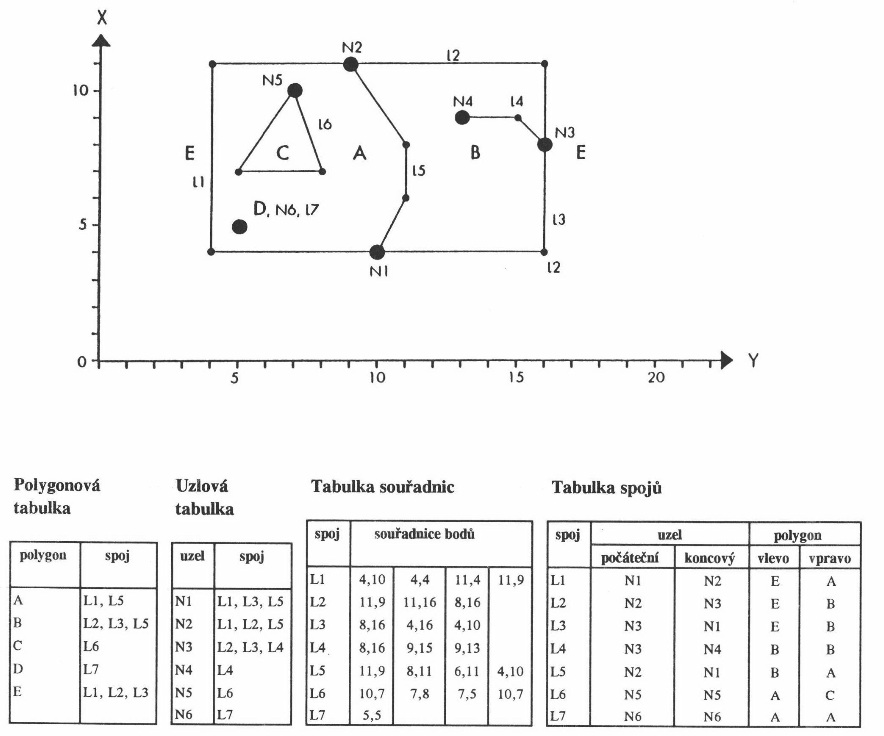
\includegraphics[width=10cm]{./pictures/3/topo_model.png}
  \caption{Ukázka topologického modelu (převzato z \cite{kolar2003geograficke})}
  \label{fig:3-time_complexity}
\end{figure}

\chapter{Navrhování algoritmů}
\label{chap:navrhovanialgoritmu}
	V této kapitole se budeme zabývat problematikou návrhu algoritmů ve výpočetní geometrii. Abychom byli schopni jednotlivé algoritmi mezi sebou porovnávat co se týče rychlosti a nároků na paměť, bude zde zmíněna asymptotická složitost. Dále zde budou představeny nejznámější techniky návrhů algoritmů ve výpočetní geometrii, které nám mohou usnadnit práci a dostat na problém jiný pohled.

\section{Časová a prostorová složitost algoritmů}
	Abychom mohli porovnávat algoritmy, řešící stejný problém, mezi sebou a rozhodnout se kdy který algoritmus použít, slouží nám k tomuto účelu základní dvě míry pro porovnání.
\begin{itemize}
	\item časová složitost
	\item prostorová složitost
\end{itemize}
	Časová složitost vyjadřuje jak dlouho bude výpočet podle daného algoritmu trvat, obdobně prostorová složitost nám vyjadřuje kolik prostoru, tedy paměti, danému algoritmu budeme muset poskytnout pro výpočet. Je očividné že vyjadřovat časovou složitost v sekundách a prostorovou v bytech by vzhledem k různému hardwaru, či různé implementaci nebylo příliš vhodné. Pro popis složitosti algoritmu tedy používáme \textit{Asymptotickou složitost}.
	
\subsection{Asymptotická složitost}
	Asymptotická složitost se vyjadřuje jako matematická funkce, popisující závislost využití paměťového prostoru nebo výpočetního výkonu na velikosti vstupních dat $N$. Důležité je že tato funkce je neklesající a vyjadřujeme ji pouze jako třídu složitosti, tedy typ funkce a ne jako přesné vyjádření. Pro příklad funkce $f(x)=1000N^2$ nebo $g(x)=N^2 + 1000N$ jsou třídy složitosti $\mathcal{O} (N^2)$. Tedy zanedbáváme multiplikativní konstantu, aditivní konstantu a nižší řády funkce, protože nás zajíma jak se bude měnit časová složitost vzhledem ke zvětšujícím vstupním datům.
	
	Tím že zanedbáváme multiplikativní, aditivní konstantu a nižší řády funkce, může se vyskytnout případ kdy algoritmus s vyžším řádem asymptotické složitosti proběhne rychleji než algoritmus s nižším řádem. Máme ovšem jistotu že existuje vstup o velikosti $N_0$, kde toto přestane platit. Při praktickém použití tato situace může nastat v případě, kdy asymptoticky rychlejší algoritmus má složitější implementaci a prostředky vynaložené na režiji převyšují výhody algoritmu. Takováto situace je vyjádřena na obrázku \ref{fig:4-time_complexity}, kde vidíme že díky zanedbaným multiplikativním a aditivním konstantám může být reálný čas výpočtu asymptoticky rychlejšího algoritmu menší než algoritmu s vyžší asymptotickou časovou složitostí. Je zde ovšem vidět že při velikosti vstupu $N_0$ se situace obrátí a dále se chovají tak, jak bysme očekávali.\cite{hartmanis1965on}
	
\begin{figure}[h]
  \centering
  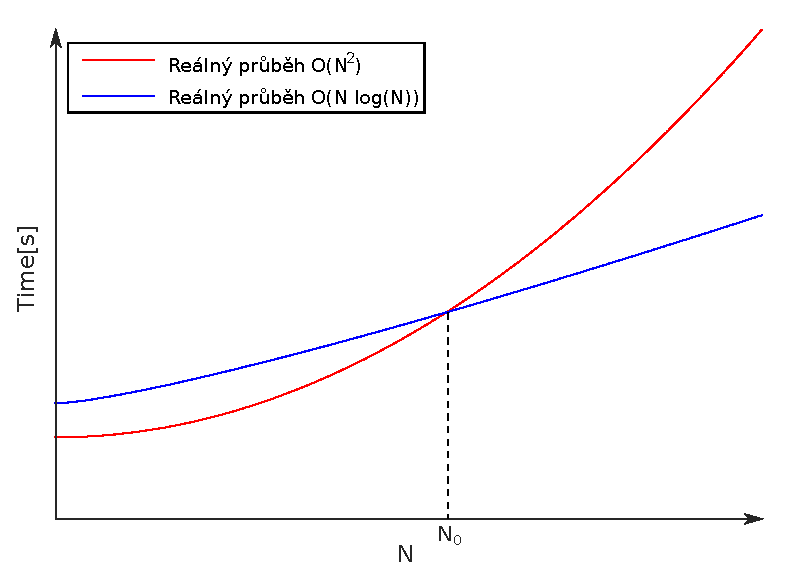
\includegraphics[width=10cm]{./pictures/4/time_complexity.pdf}
  \caption{Graf znázorňující časový průběh algoritmu v závislosti na velikosti vstupu $N$}
  \label{fig:4-time_complexity}
\end{figure}
	
	 Pro vyjádření časové složitosti můžeme využít různé varianty.
\begin{itemize}
	\item Horní odhad složitosti - $\mathcal{O} (f(N))$
	\item Průměrná složitost - $\Theta (f(N))$
	\item Dolní odhad složitosti - $\Omega (f(N))$
\end{itemize}	
	Často vídané vyjádření složitosti je takzvaná \textit{Omikron notace}, která vyjadřuje horní odhad, tedy nejhorší možný případ jakým se může algoritmus chovat. V tomto případě máme jistotu že algoritmus bude asymptoticky probíhat stejně rychle nebo rychleji v případě časové složitosti. V některých případech se vyplatí uvádět i průměrnou složitost, tedy složitost, která nastává při náhodném rozložení vstupních dat. Typickou ukázkou, kde je vhodné využít průměrnou časovou složitost je metoda \textit{Quick-Sort}, která patří mezi třídící algoritmy. Horní odhad složitosti je $\mathcal{O}(n^2)$. Při vhodné implementaci se ovšem lze kvadratické složitosti účinně bránit a obecně se algoritmus chová s průměrnou časovou složitostí $\Theta (n \log n)$ což je pro třídící algoritmy nejlepší možné.\cite{wirth1989algoritmy} Poslední variantou je dolní odhad složitosti, který nám naopak vyjadřuje že algoritmus se bude chovat stejně nebo hůře než je uvedeno. Toto vyjádření využijeme především v oblasti kryptografie.\cite{milkova2010algoritmy} \cite{bayer2008algoritmy}
	
\subsection{Stanovení časové složitosti}
	Pro určení časové složitosti je nutné určit počet operací v závislosti na velikosti vstupních dat. Nezajímame se o přesný počet operací, ale o vztahu počtu operací k velikosti vstupní množiny. Pro komplikované algoritmy to může být nesnadný úkol. U geometrických algoritmů se často zajímáme pouze o horní odhad složitosti, díky jeho relativně jednoduchému zjištění oproti průměrnému odhadu.
	
	
\begin{table}

\begin{tabular}{ |p{1.4cm}||p{1.6cm}|p{1.6cm}|p{1.6cm}|p{1.6cm}|p{1.6cm}|p{1.6cm}|  }
% \hline
% \multicolumn{7}{|c|}{Závislost času výpočtu na asymptotické složitosti} \\
\hline

$N$				&10			&20			&40			&60			&500		&1000\\
\hline
$\log n$		&2,3µs		&4,3µs		&5µs		&5,8µs		&9µs		&10µs\\			
$n$				&10µs		&20µs		&40µs		&60µs		&0,5s		&1ms\\
$n \log n$		&23µs		&86µs		&0,2ms		&0,35ms		&4,5ms		&10ms\\
$n^2$			&0,1ms		&0,4ms		&1,6ms		&3,6ms		&0,25s		&1s\\
$n^3$			&1ms		&8ms		&64ms		&0,2s		&125s		&17min\\
$n^4$			&10ms		&160ms		&2,56s		&13s		&17h		&11,6dní\\
$2^n$			&1ms		&1s			&12,7 dní	&36000 let	&			&\\
$n!$			&3,6s		&77000 let	&			&			&			&\\
\hline

\end{tabular}
\caption{Příklad závislosti výpočetního času na asymptotické složitosti algoritmu}
\label{tab:4-time_complexity}
\end{table}

\section{Metody návrhů algoritmů ve výpočetní geometrii}
	Abychom byli schopni porozumět různým algoritmům, nebo navrhnout nový algoritmus pro různé operace ve výpočetní geometrii, je dobré seznámit se s často využívanými metodami, používané v algoritmech výpočetní geometrie. Metody návrhů alogritmů neřeší konkrétní problém, ale pouze obecný postup jak se při hledání řešení chovat.

\subsection{Metoda hrubé síly}
	Patří k nejjednodušším metodám algoritmizace. Jak vyplývá z názvu, v této metodě budeme postupovat hrubou silou, tedy v praxi to znamená že algoritmus bude zkoušet všechny možné kombinace řešení. Mezi výhody patří jednoduchá implementace a snadné porozumění algoritmu, které se často shoduje s definicí výsledku. Tyto algoritmy lze využívat zpravidla pro malé vstupní množiny, nebo pro ověření správnosti výsledku. V praxi lze algoritmy využít i jako doplněk složitějších algoritmů, kde by režije, jako je volání funkcí nebo vytváření objektů, zabralo více času než na tuto malou množinu použít algoritmus hrubé síly. Velmi často je časová složitost těchto algoritmů $\mathcal{O}(2^n)$ či dokonce $\mathcal{O}(n!)$. V tabulce \ref{tab:4-time_complexity} pak můžeme vidět že časová složitost pro větší vstupy je neúnosná.
	
\subsection{Heuristické algoritmy}
	Heuristické algoritmy se velmi podobají metodě hrubé síly, pouze nezkoumají všechna možná řešení. Tato technika je velmi často používaná u optimalizačních úloh, kde neexistuje exaktní řešení. Zatím co u algoritmu řešící úlohu metodou hrubé síly bylo nalezení optimálního řešení zaručeno, heuristické algoritmy hledají pouze přípustné řešení. Tímto způsobem docílíme lepší časové náročnosti oproti algoritmům hrubé síly. Jednou ze známých metod heuristických algoritmů jsou takzvané hladové algoritmy. Ty se nalezením lekálně optimálních řešení snaží docílit lokálního optima. Příkladem hladového algoritmu může být nalezení nepravidelné trojúhelníkové sítě nad množinou bodů v rovině, kdy postupně přidáváme do řešení nejkratší hrany, pokud ovšem nekříží jinou hranu vyskytující se již v řešení.
	
\begin{figure}[h]
    \centering % <-- added
\begin{subfigure}{0.25\textwidth}
  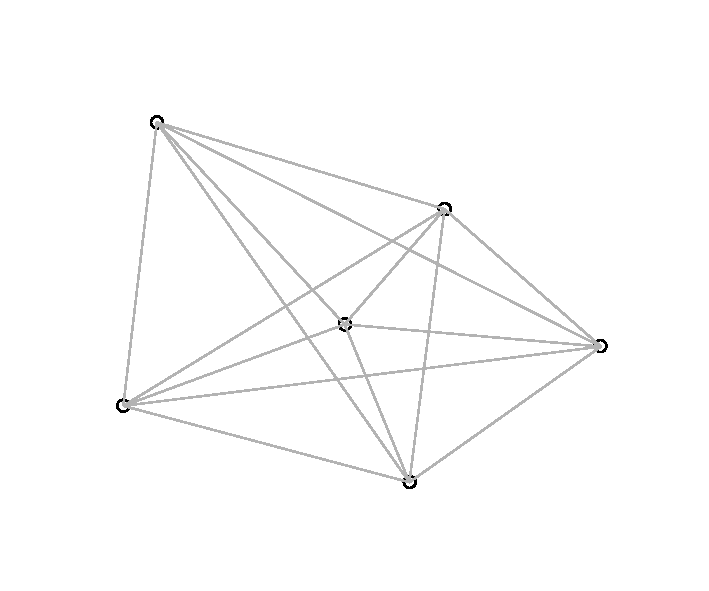
\includegraphics[width=\linewidth]{./pictures/4/triangulation_1.pdf}
  \label{fig:3-triangulation_1}
\end{subfigure}\hfil % <-- added
\begin{subfigure}{0.25\textwidth}
  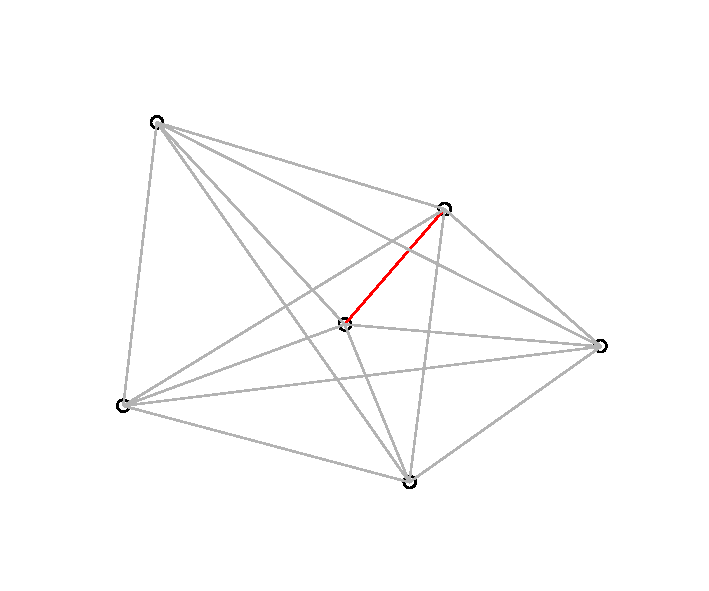
\includegraphics[width=\linewidth]{./pictures/4/triangulation_2.pdf}
  \label{fig:3-triangulation_2}
\end{subfigure}\hfil % <-- added
\begin{subfigure}{0.25\textwidth}
  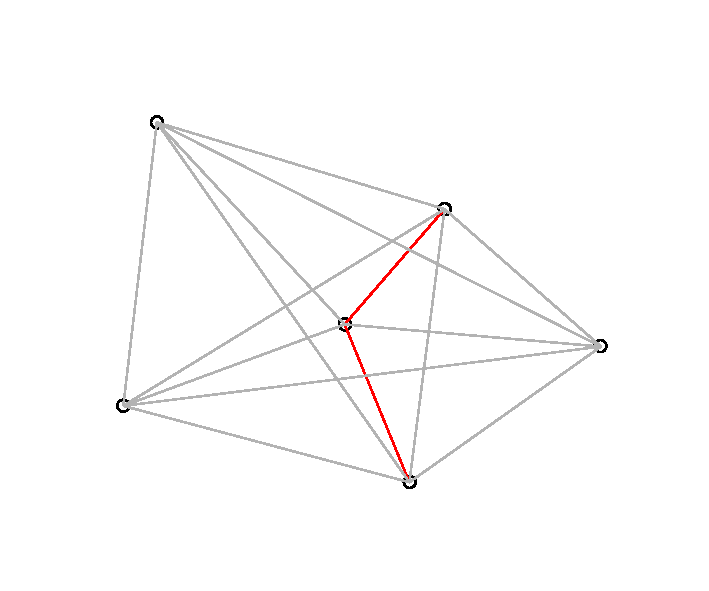
\includegraphics[width=\linewidth]{./pictures/4/triangulation_3.pdf}
  \label{fig:3-triangulation_3}
\end{subfigure}\hfil % <-- added
\begin{subfigure}{0.25\textwidth}
  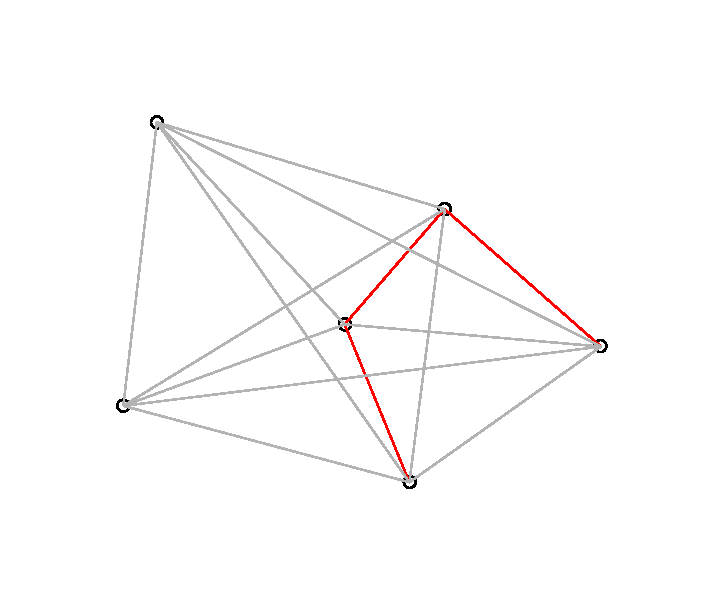
\includegraphics[width=\linewidth]{./pictures/4/triangulation_4.pdf}
  \label{fig:3-triangulation_4}
\end{subfigure}\hfil % <-- added
\begin{subfigure}{0.25\textwidth}
  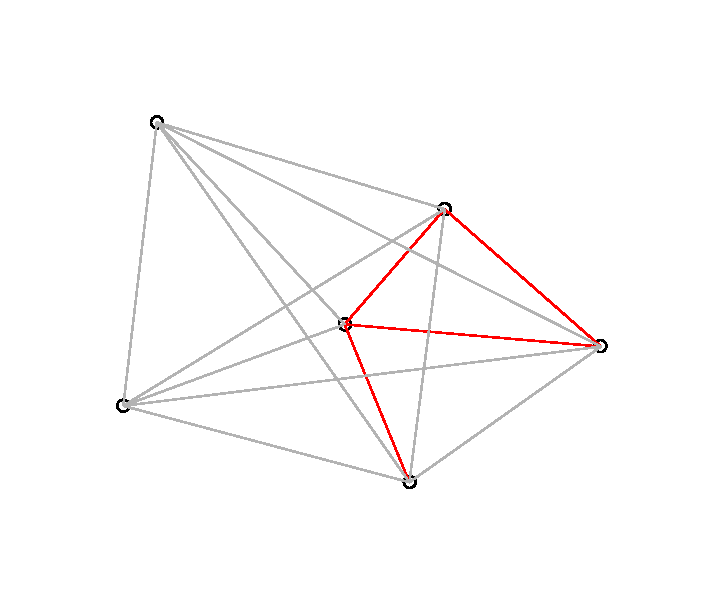
\includegraphics[width=\linewidth]{./pictures/4/triangulation_5.pdf}
  \label{fig:3-triangulation_5}
\end{subfigure}\hfil % <-- added
\begin{subfigure}{0.25\textwidth}
  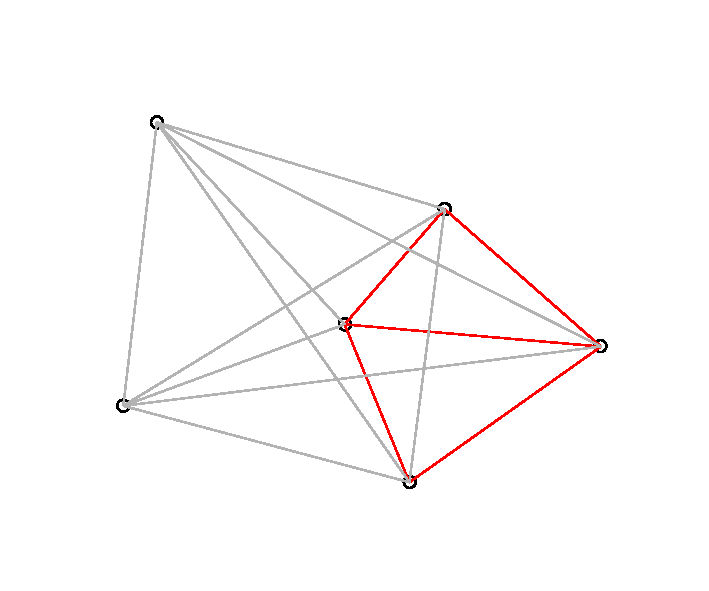
\includegraphics[width=\linewidth]{./pictures/4/triangulation_6.pdf}
  \label{fig:3-triangulation_6}
\end{subfigure}\hfil % <-- added
\begin{subfigure}{0.25\textwidth}
  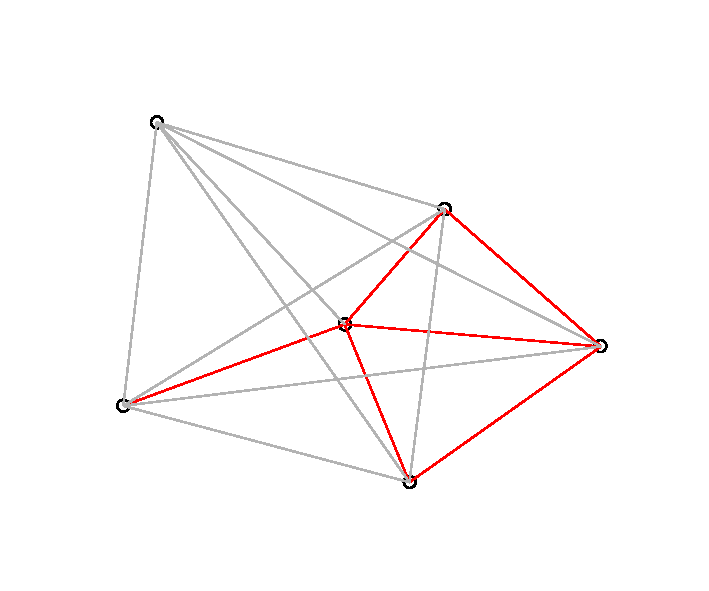
\includegraphics[width=\linewidth]{./pictures/4/triangulation_7.pdf}
  \label{fig:3-triangulation_7}
\end{subfigure}\hfil % <-- added
\begin{subfigure}{0.25\textwidth}
  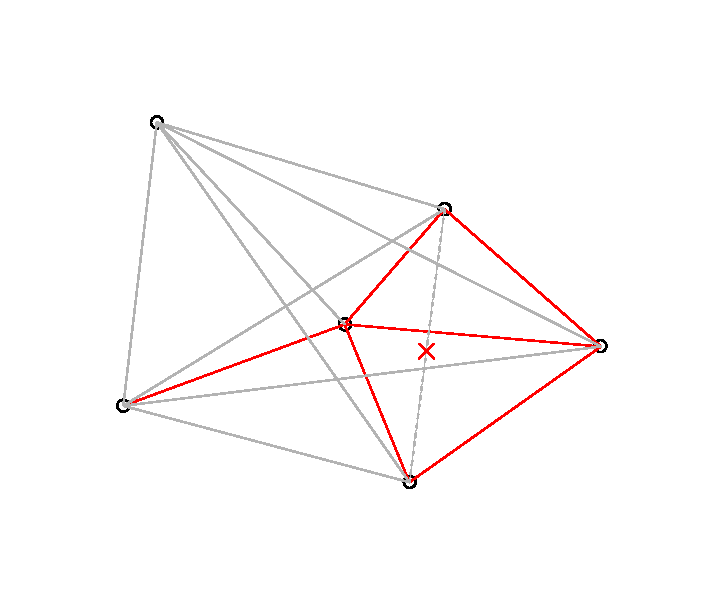
\includegraphics[width=\linewidth]{./pictures/4/triangulation_8.pdf}
  \label{fig:3-triangulation_8}
\end{subfigure}\hfil % <-- added
\begin{subfigure}{0.25\textwidth}
  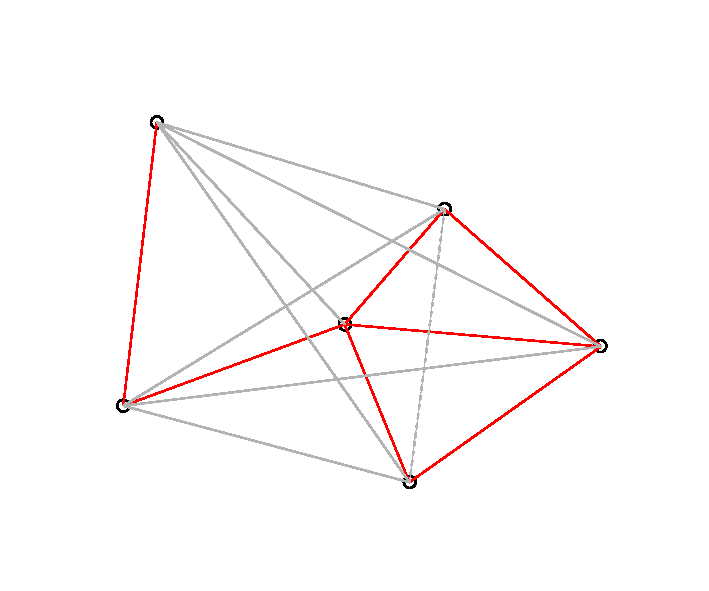
\includegraphics[width=\linewidth]{./pictures/4/triangulation_9.pdf}
  \label{fig:3-triangulation_9}
\end{subfigure}\hfil % <-- added
\begin{subfigure}{0.25\textwidth}
  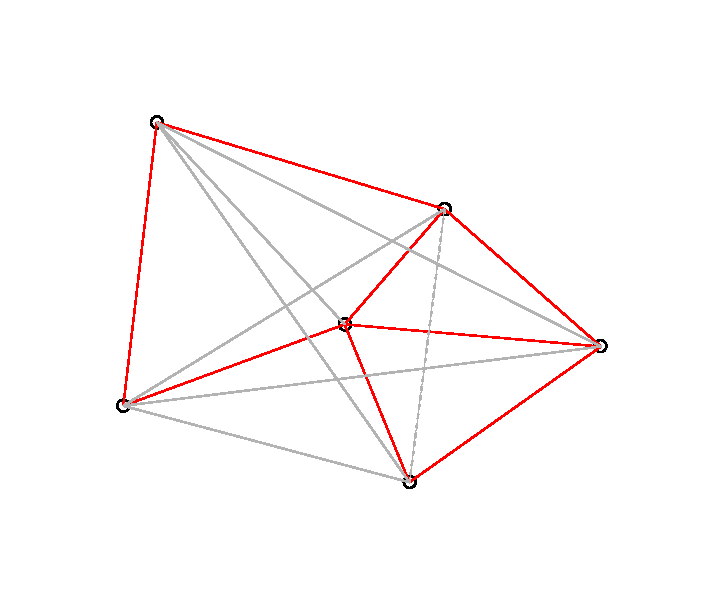
\includegraphics[width=\linewidth]{./pictures/4/triangulation_10.pdf}
  \label{fig:3-triangulation_10}
\end{subfigure}\hfil % <-- added
\begin{subfigure}{0.25\textwidth}
  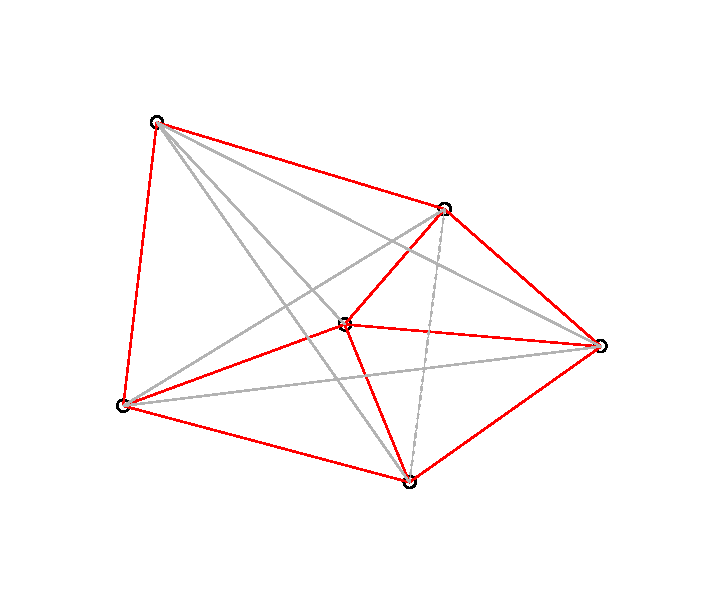
\includegraphics[width=\linewidth]{./pictures/4/triangulation_11.pdf}
  \label{fig:3-triangulation_11}
\end{subfigure}\hfil % <-- added
\begin{subfigure}{0.25\textwidth}
  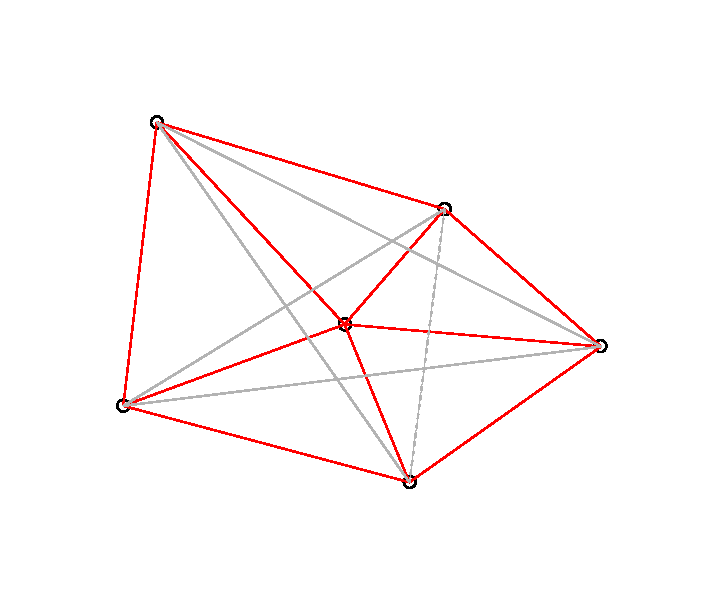
\includegraphics[width=\linewidth]{./pictures/4/triangulation_12.pdf}
  \label{fig:3-triangulation_12}
\end{subfigure}\hfil % <-- added

\caption{Znázornění postupu algoritmu pro nalezení triangulace metodou hladového algoritmu.}
\label{fig:3-triangulation}
\end{figure}	
	
	
	
\subsection{Rozděl a panuj}
	Nejen ve výpočetní geometrii je známá a hojně používaná metoda \textit{rozděl a panuj}, známá také pod anglickým názvem \textit{divide and conquer}. Paradigma je založeno na rekurzivním rozdělování problému na dvě či více částí, stejného nebo podobného typu, dokud nebudeme schopni problém jednoduše vyřešit. Řešení dílčích problémů se pak spojuje a získá se řešení původního problému. Metoda \textit{rozděl a panuj} je vhodná pro paralelní zpracování, kde pří každém rozdělení nám vznikají dvě či více částí, které můžeme řešit nezávisle na sobě.\cite{frigo1999cache}
	Do algoritmů této kategorie patří například generalizační algoritmus \textit{Douglas-Peucker}\cite{van1997algorithmic}, který je vhodný svou jednoduchostí na ukázkou metody rozděl a panuj. 
	Na vstupu dostává algoritmus linii, kterou chceme generalizovat a hodnotu vzdálenosti o kterou se generalizovaná linie může maximálně lišit od původní. Funkce vyhledá bod s maximální vzdáleností od úsečky spojující počáteční a koncový bod, který je zároveň vzdálenější než námi zadaná mez, poté se rekurzivně zavolá na dvě úsečky obsahující tento bod. Takto se postupuje do té doby dokud existuje bod s větší vzdáleností než zadaná mez. Po dokončení se řešení složí z jednotlivých kroků rekurze.

\begin{figure}[h]
    \centering % <-- added
\begin{subfigure}{0.5\textwidth}
  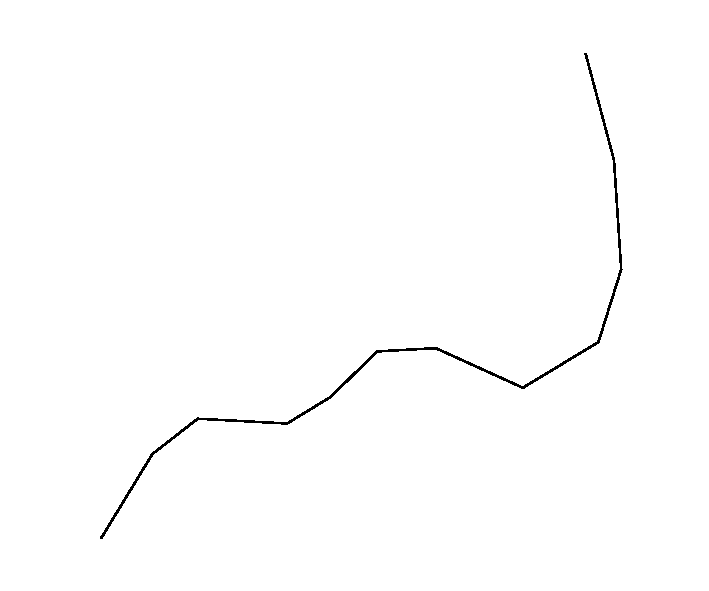
\includegraphics[width=\linewidth]{./pictures/4/douglas-peucker_1.pdf}
  \label{fig:3-douglas-peucker_1}
\end{subfigure}\hfil % <-- added
\begin{subfigure}{0.5\textwidth}
  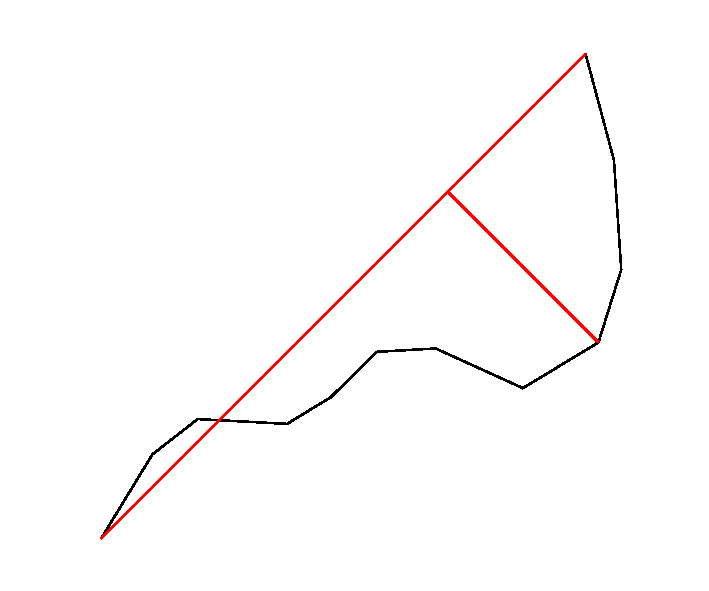
\includegraphics[width=\linewidth]{./pictures/4/douglas-peucker_2.pdf}
  \label{fig:3-douglas-peucker_2}
\end{subfigure}\hfil % <-- added
\begin{subfigure}{0.5\textwidth}
  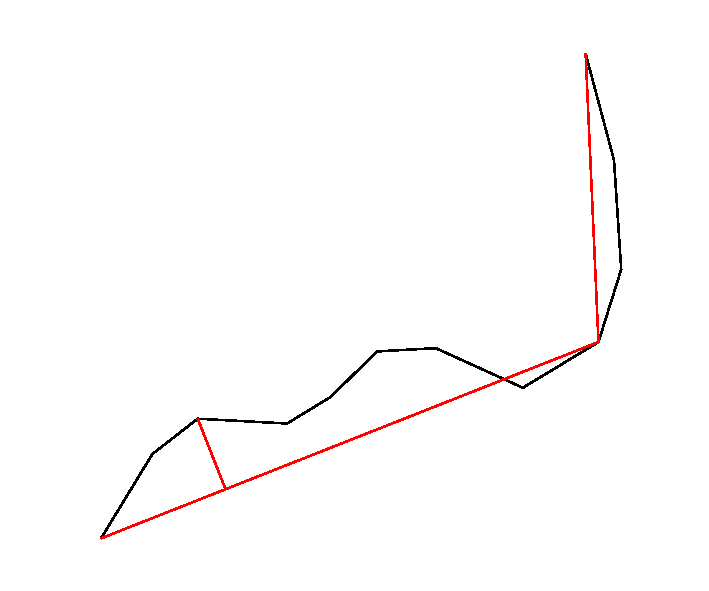
\includegraphics[width=\linewidth]{./pictures/4/douglas-peucker_3.pdf}
  \label{fig:3-douglas-peucker_3}
\end{subfigure}\hfil % <-- added
\begin{subfigure}{0.5\textwidth}
  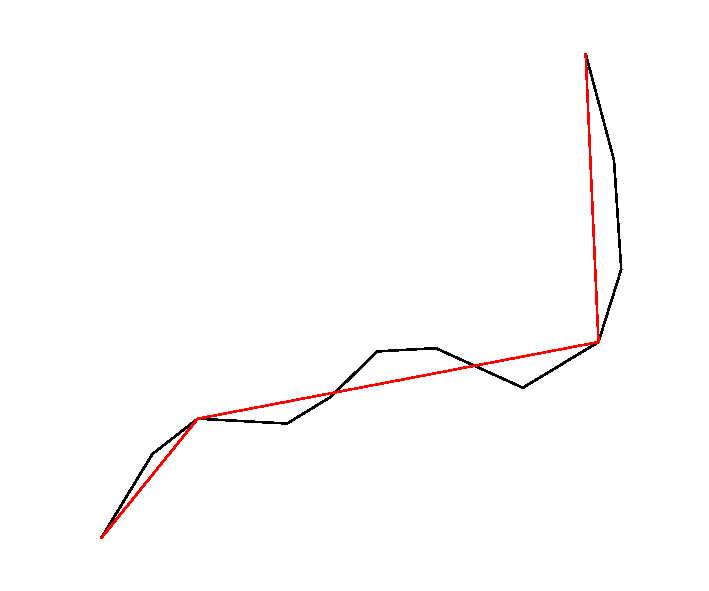
\includegraphics[width=\linewidth]{./pictures/4/douglas-peucker_4.pdf}
  \label{fig:3-douglas-peucker_4}
\end{subfigure}\hfil % <-- added
\caption{Znázornění postupu \textit{Douglas-Peucker} algoritmu pro ukázku metody \textit{rozděl a panuj}}
\label{fig:3-douglas-peucker}
\end{figure}
	

\subsection{Zametací přímka}
	Další metoda využívaná výhradně ve výpočetní geometrii je metoda takzvané \textit{zametací přímky}, neboli \textit{sweep line}. Myšlenkou této techniky je procházení setříděných dat. Ve výpočetní geometrii se nejčastěji jedná o průchod bodů seřazených podle jedné ze souřadnic. Pokud takto setříděnou vstupní množinou nedisponujeme, je nutno nejprve data setřídit jedním ze známích třídících algoritmů. Pak lze průchod body vizualizovat, podle implementace, například jako svislou přímku pohybující se z leva do prava po množině bodů.
	Tuto metudu využívá například \textit{Bentley-Ottmannův} algoritmus pro nalezení průsečíků množin linií, který je podrobněji popsán v kapitole \ref{chap:reserzepouzivanychalgoritmu}, proto se jím zde nebudeme zabývat.

\subsection{Inkrementální algoritmy}
	Algoritmy tohoto typu se snaží dosáhnout výsledku tím způsobem, že ze vstupní množiny přidávájí, nebo aktualizují prvky ve výstupní množině. Tedy po každém kroku je řešení aktualizováno dokud není dosaženo konečného výsledku. Výhodou této metody je že často lze použít pro online algoritmy, tedy do vstupní množiny mohou být přidávány prvky v průběhu výpočtu.
	Pro ukázku zde byl vybrán algoritmus pro inkrementální výpočet konvexní obálky. Algoritmus vybere bod ze vstupní množiny a určí polohu vůči aktuálním liniím konvexní obálky. Pokud bod vůči nějakým hranám leží v pravé polorovině, tyto hrany jsou označeny čárkovaně, algoritmus odebere tyto hrany z konvexní obálky a mezi volné konce přidá aktuálně zkoumaný bod. Pokud bod leží vůči všem hranám v levé polorovině, řešení se neaktualizuje a pokračuje se dál. Na tomto příkladu je vidět i možnost využívat algoritmus online, tedy kdykoliv do výpočtu zahrnout další body.

\begin{figure}[h]
    \centering % <-- added
\begin{subfigure}{0.5\textwidth}
  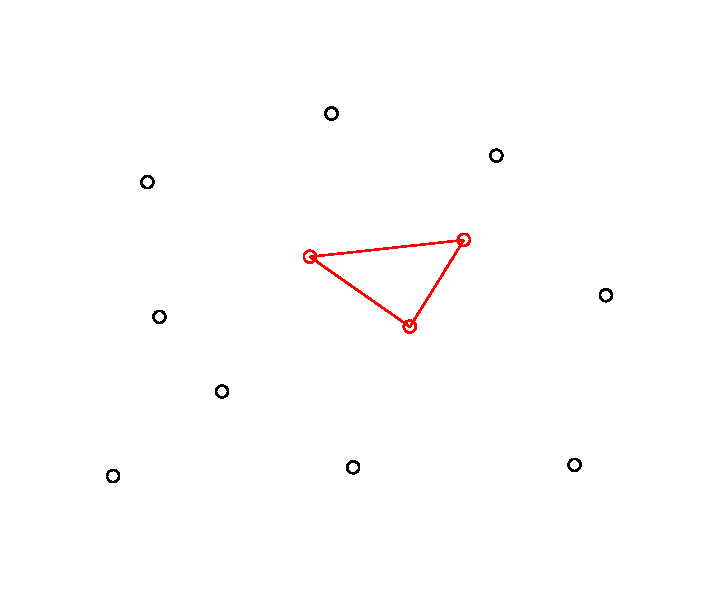
\includegraphics[width=\linewidth]{./pictures/4/incremental_hull_1.pdf}
  \label{fig:3-douglas-peucker_1}
\end{subfigure}\hfil % <-- added
\begin{subfigure}{0.5\textwidth}
  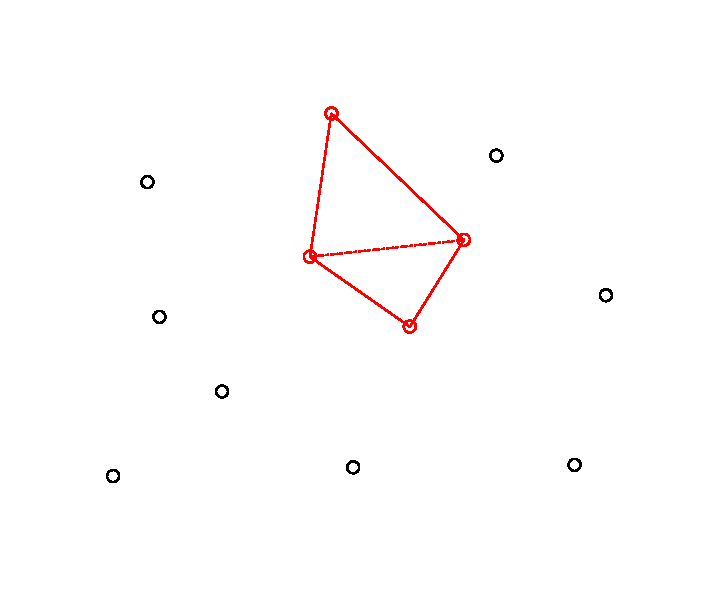
\includegraphics[width=\linewidth]{./pictures/4/incremental_hull_2.pdf}
  \label{fig:3-douglas-peucker_2}
\end{subfigure}\hfil % <-- added
\begin{subfigure}{0.5\textwidth}
  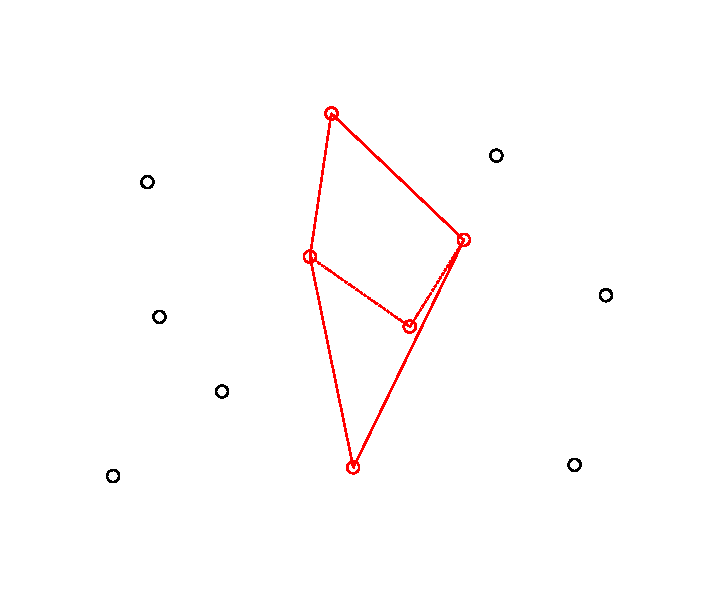
\includegraphics[width=\linewidth]{./pictures/4/incremental_hull_3.pdf}
  \label{fig:3-douglas-peucker_3}
\end{subfigure}\hfil % <-- added
\begin{subfigure}{0.5\textwidth}
  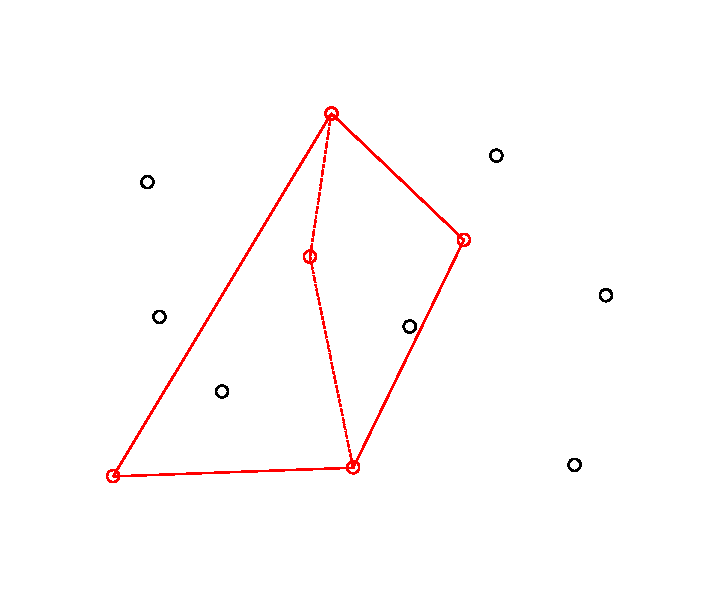
\includegraphics[width=\linewidth]{./pictures/4/incremental_hull_4.pdf}
  \label{fig:3-douglas-peucker_4}
\end{subfigure}\hfil % <-- added
\caption{Znázornění postupu inkrementálního algoritmu pro konvexní obálku}
\end{figure}
\chapter{Rešerše používaných algoritmů}
\label{chap:reserzepouzivanychalgoritmu}
	Tato kapitola se zabývá přehledem využívaných algoritmů pro tvorbu polygonů z množiny linií. Polygonizace, tak jak jí můžeme pozorovat v různých GIS softwarech, se zpravidla neřeší jedním algoritmem, ale používají se různé algoritmy pro jednotlivé kroky polygonizace. Popíšeme zde tedy do jakých kroků lze polygonizaci rozdělit a jak jednotlivé kroky optimálně řešit. Budeme se zabývat i řešením v jednotlivých GIS softwarech.

	Polygonizaci lze nejjednodušeji rozdělit na 2 základní kroky. Jako vstupní data budeme uvažovat množinu linií, tyto linie ovšem nemusí obsahovat, v reálném použití převážně neobsahují, lomové body ve společných průsečících. Tato situace nastává především použiváme-li různé vrstvy pro tvorbu polygonů. V terminologii GIS se tyto průsečíky označují jako \textit{fuzzy}, volně přeloženo jako \textit{neostré}. Abychom mohli zahájit další krok polygonizace, je nutné tyto průsečíky doplnit. V první části se tedy budeme zabývat, jak optimálně doplnit průsečíky množin linií.
	
	Předpokládejme že množina linií je zbavená \textit{fuzzy} průsečíků, tedy každá dvojice úseček má společný nanejvýš jeden koncový bod. V takovéto situaci můžeme přistoupit k dalšímu kroku, tedy vlastní tvorbě polygonů z množiny linií. Polygony, které hledáme, musí splňovat podmínku, že žádný námi vytvořený polygon nemůže být rozdělen jakoukoliv linií na více menších polygonů. Pro řešení tvorby polygonů se často využívá grafových algoritmů.
	
\begin{figure}[h]
    \centering % <-- added
\begin{subfigure}{0.5\textwidth}
  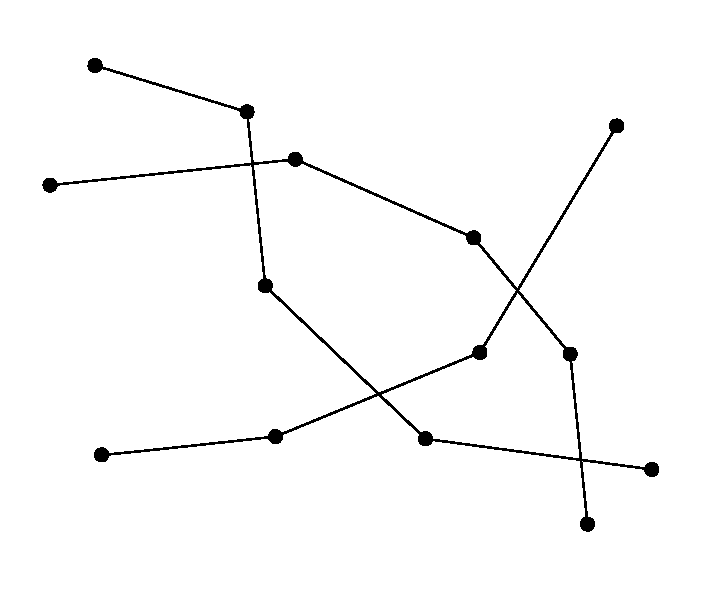
\includegraphics[width=\linewidth]{./pictures/5/fuzzy_1.pdf}
  \caption{Množina linií s fuzzy průsečíky}
  \label{fig:2-fuzzy_1}
\end{subfigure}\hfil % <-- added
\begin{subfigure}{0.5\textwidth}
  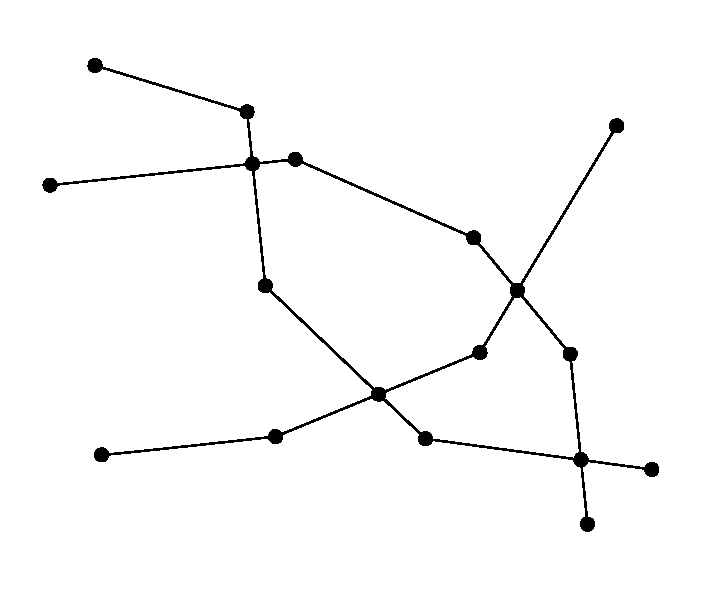
\includegraphics[width=\linewidth]{./pictures/5/fuzzy_2.pdf}
  \caption{Množina linií doplněná o průsečíky}
  \label{fig:2-fuzzy_2}
\end{subfigure}\hfil % <-- added
\begin{subfigure}{0.5\textwidth}
  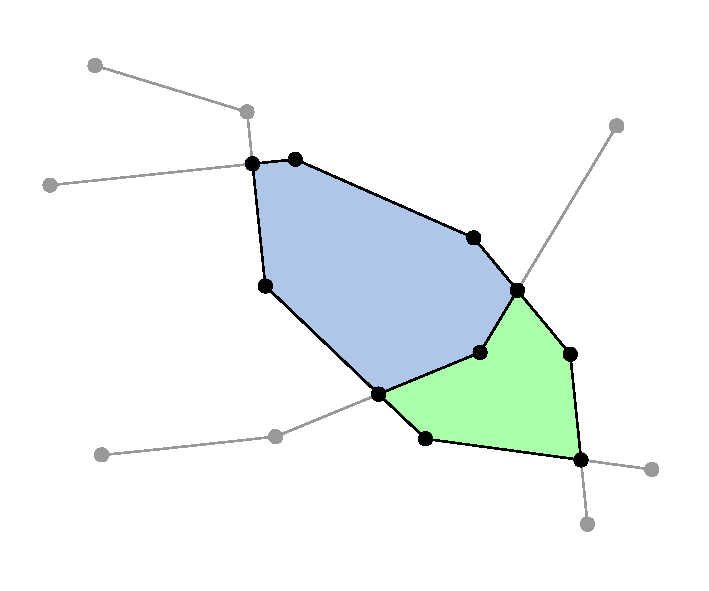
\includegraphics[width=\linewidth]{./pictures/5/fuzzy_3.pdf}
  \caption{Vytvořené polygony}
  \label{fig:2-fuzzy_2}
\end{subfigure}\hfil % <-- added
\caption{Znázornění postupu polygonizace}
\end{figure}

\section{Výpočet průsečíků množiny linií}
Výpočet všech průsečíků množin linií lze provést snadno, testováním všech úseček se všemi. Tímto postupem ovšem zjevně dosáhneme složitosti $\mathcal{O}(N^2)$ kde $N$ je počet úseček. Pro výpočet průsečíků lze ovšem využít i algoritmus s časovou náročnosti $\mathcal{O}(n\log{}n)$, známý také jako Bentley–Ottmannův algoritmus \cite{bentley1979algorithms}.

\subsection{Vzájemná poloha dvou úseček}
Ve 2D výpočetní geometrii jsou standardně jednotlivé segmenty linie vyjádřeny počátečními a koncovými souřadnicemi. Uvažujme tedy že máme dány 2 přímky $p_1 = |S_1 E_1|$ a $p_2 = |S_2 E_2|$, kde $S_1 = [x_{S1},y_{S1}]$, $E_1 = [x_{E1},y_{E1}]$, $S_2 = [x_{S2},y_{S2}]$, $E_2 = [x_{E2},y_{E2}]$ a potřebujeme provést test, zda se dané přímky protínají či nikoliv, můžeme použít takzvaný \textit{Half-Plane} test, tedy test, který určuje zda bod leží v pravé či levé polorovině od přímky. Tento test zopakujeme celkem čtyřikrát a to na počáteční a koncový bod druhé úsečky, abysme zjistili zda se přímky protínají. Test je založen na výpočtu orientace dvou vektorů $\vec{u}$  a $\vec{v}$, kde vektor $\vec{u}$ je směrový vektor úsečky, tedy $\overrightarrow{S_1E_1}$ a vektor $\vec{v}$ je vektor $\overrightarrow{S_1S_2}$. Po aplikaci výpočtu orientace vektorů na každý z koncových bodů jsme schopni jednoduše určit zda se dané přímky protínají. Tento postup nám ovšem nedá souřadnice samotného průsečíku.

\begin{figure}[h]
  \centering
  \includegraphics[width=7.5cm]{./pictures/5/half-plane_vector.pdf}
  \caption{\textit{Half-plane} test}
  \label{fig:2-half_plane_vector}
\end{figure}

\begin{figure}[h]
    \centering % <-- added
\begin{subfigure}{0.5\textwidth}
  \includegraphics[width=\linewidth]{./pictures/5/half-plane_1.pdf}
  \caption{Test bodu $S_2$ k přímce $|S_1E_1|$}
  \label{fig:2-half_plane_1}
\end{subfigure}\hfil % <-- added
\begin{subfigure}{0.5\textwidth}
  \includegraphics[width=\linewidth]{./pictures/5/half-plane_2.pdf}
  \caption{Test bodu $E_2$ k přímce $|S_1E_1|$}
  \label{fig:2-half_plane_2}
\end{subfigure}\hfil % <-- added

\medskip
\begin{subfigure}{0.5\textwidth}
  \includegraphics[width=\linewidth]{./pictures/5/half-plane_3.pdf}
  \caption{Test bodu $S_1$ k přímce $|S_2E_2|$}
  \label{fig:2-half_plane_3}
\end{subfigure}\hfil % <-- added
\begin{subfigure}{0.5\textwidth}
  \includegraphics[width=\linewidth]{./pictures/5/half-plane_4.pdf}
  \caption{Test bodu $E_1$ k přímce $|S_2E_2|$}
  \label{fig:2-half_plane_4}
\end{subfigure}\hfil % <-- added
\caption{Grafické znázornění \textit{Half-plane} testů pro zjištění existence průsečíku}
\label{fig:2-half_plane}
\end{figure}

\subsection{Nalezení průsečíku dvou úseček}
	Pro nalezení průsečíku $P$ dvou úseček vycházíme z parametrického vyjádření přímek, jelikož obecné rovnice neumožňují pracovat s přímkami rovnoběžnými s osou y. Uvažujme tedy stejné značení bodů jako v předchozím odstavci. Nejprve je tedy nutné vyjádřit rovnici přímky z počátečního a koncového vrcholu. Pro parametrické vyjádření využijeme směrový vektor přímky a libovolný bod na přímce. Ovšem pro zjednodušení výpočtů použijeme pro přímku $p_1$ směrový vektor $\overrightarrow{S_1E_1}$ a jako bod do parametrické rovnice dosadíme $S_1$, obdobně zkonstruujeme i parametrické vyjádření přímky $p_2$. Soustava rovnic pro výpočet průsečíku $p_i$ pak tedy bude vypadat takto:
	
\begin{align*} 
P = S_1 + s \cdot \overrightarrow{S_1E_1}, \\
P = S_2 + t \cdot \overrightarrow{S_2E_2}. \\
\end{align*}

Rozepsáno podle souřadnic:

\begin{align*} 
x_P = x_{S1} + s(x_{E1} - x_{S1}), \\
y_P = y_{S1} + s(y_{E1} - y_{S1}), \\
x_P = x_{S2} + t(x_{E2} - x_{S2}), \\
y_P = y_{S2} + t(y_{E2} - y_{S2}).
\end{align*}

Pro získání průsečíku musíme nejprve ze soustavy rovnic vyjádřit parametry $s$ a $t$. To provedeme následujícím způsobem:

\begin{align*} 
s = \frac{y_{S1}(x_{S2} - x_{E2}) + y_{S2}(x_{E2} - x_{S1}) + y_{E2}(x_{S1} - x_{S2})}{(x_{E1} - x_{S1}) (y_{S2} - y_{E2})   -   (y_{E1} - y_{S1}) (x_{S2} - x_{E2})}, \\
t = \frac{y_{S1}(x_{S2} - x_{E1}) + y_{E1}(x_{S1} - x_{S2}) + y_{S2}(x_{E1} - x_{S1})}{(x_{E1} - x_{S1}) (y_{S2} - y_{E2})   -   (y_{E1} - y_{S1}) (x_{S2} - x_{E2})}.
\end{align*}


Z charakteru parametrického vyjádření přímek poté můžeme rozhodnout o vzájemné poloze úseček. Pokud parametry $s \in <0,1>, t \in <0,1>$ pak se úsečky protínají, v opačném případě se úsečky neprotínají. Je potřeba ošetřit případy kdy úsečky leží na jedné přímce.


\subsection{Bentley–Ottmannův algoritmus}
Tento algoritmus je založen na technice zvané \textit{sweep line} neboli \textit{zametací přímka}. Tato technika je již zmíněna v kapitole \ref{chap:navrhovanialgoritmu}. Hlavní myšlenka pro zrychlení algoritmu oproti metodě hrubé síly je počítat průsečíky pouze sousedních linií, tedy linií které jsou právě protnuty zametací přímkou.

prioritní fronta - seřazené body podle jedné ze souřadnic





, podle jedné ze souřadnic. Algoritmus zde nebuda více popisován jelikož je velmi dobře vysvětlen v těchto publikacích \cite{bentley1979algorithms} \cite{bayer2008algoritmy}.
% https://www.cs.princeton.edu/~rs/AlgsDS07/17GeometricSearch.pdf
% https://courses.csail.mit.edu/6.006/spring11/lectures/lec24.pdf
% https://cw.fel.cvut.cz/old/_media/courses/ae4m39vg/lectures/09-intersect.pdf





\section{Tvorba polygonů z množiny linií}
Předpokládejme že máme množinu linií doplněnou o průsečíky, tedy každá dvojice úseček v této množině sdílí nejvýše jeden koncový bod. V předchozí sekci bylo řečeno že průsečíky linií lze doplnit pomocí \textit{Bentley–Ottmannova} algoritmu v čase $\mathcal{O}(n\log{}n)$. Nyní chceme tedy v této množině linií nalézt všechny polygony, tak aby jednotlivé polygony spolu sdílely maximálně hrany a zároveň aby žádný z polygonů nemohl obsahovat jiný polygon. Takové linie jsou v podstatě reprezentací grafu. K nalezení polygonů můžeme použít tedy grafových algoritmů. 
	
\subsection{Dijkstrův algoritmus}


\chapter{Konvenční prostředky a polygonizace}
\label{chap:konvencni prostredky a polygonizace}
	Existuje celá řada konvenčních nástrojů, kterými lze řešit polygonizaci. Oblast GIS je známá značným množstvím kvalitních nástrojů s otevřeným zdrojovým kódem. Můžeme tak nalédnout do implementace jednotlivých softwarových řešení. Výhodou je i velká komunita, která vždy ochotně poradí. Mimo jiné jsou zde i komerční zástupci, kteří nám možnost nahlédnout do zdrojového kódu zpravidla nenabídnou. Zato by nám měli poskytovat uživatelskou podporu, za kterou zákazník samozřejmě platí koupí softwaru.
	
	Mohlo by se zdát, že nástrojů existuje celá řada, tak proč vytvářet nástroj nový? Jedná se zde především o spolehlivost a jednoduchost. Jak u komerčních, tak u open source nástrojů je s nadsázkou téměř tradicí, že po přechodu na vyšší verzi nějaké komponenty přestanou fungovat a končí na neočekávaných chybách. Výjimkou nejsou ani nástroje pro polygonizaci.
	
	Zmíníme zde tedy nejvýznamější zástupce z oblasti GIS a ukážeme, které nástroje z těchto softwarů lze pro polygonizaci využít.
	
\section{ArcGIS Desktop}
	ArcGIS je vyvíjený společností Esri, v současné době se jedná o jeden z nejvyužívanějších nástrojů v oblasti GIS. Jedná se o placený software, za který nekomerční uživatel v současné chvíli zaplatí 100 dolarů ročně. Používat tento nástroj tedy pouze pro polygonizaci by bylo nesmyslné, ovšem pokud uživatel již tímto softwarem disponuje, je toto jedna z možností.
	
\subsubsection{Feature to Polygon}
	\textit{Feature to Polygon} je nástroj sloužící pro tvorbu polygonů. Jako vstupní data mohou být použity linie i polygony. Výstupní polygony z tohoto nástroje na testovacích datech byli korektní, ovšem při větším množství vstupních linií testovaný nástroj končil chybou. Nutno podotknout, že u různých verzí softwaru se může nástroj chovat jinak.

\begin{figure}[h]
  \centering
  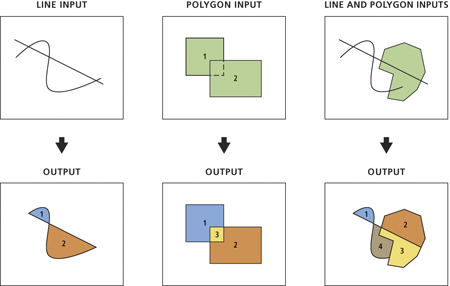
\includegraphics[width=10cm]{./pictures/5.1/feature_to_polygon.png}
  \caption{Ilustrace vstupu a výstupu nástroje Feature to Polygon. Převzato z~\cite{arcgis}.}
  \label{fig:feature_to_polygon}
\end{figure}

\begin{figure}[h]
  \centering
  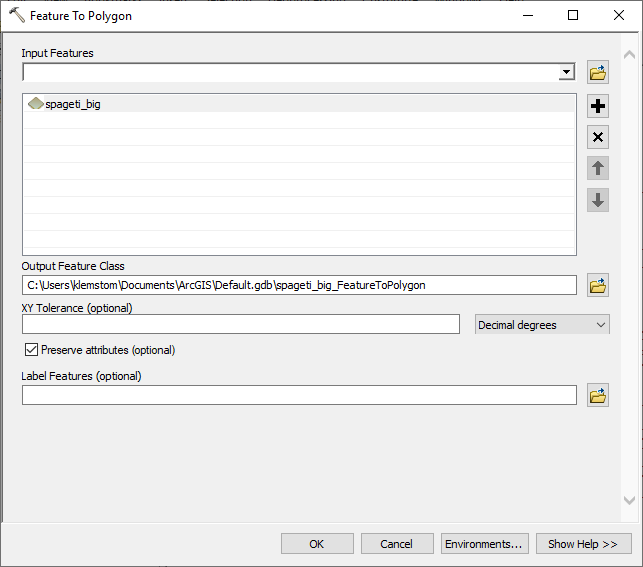
\includegraphics[width=10cm]{./pictures/5.1/feature_to_polygon-1.png}
  \caption{Rozhraní nástroje Feature to Polygon v softwaru ArcGIS Desktop.}
  \label{fig:feature_to_polygon-1}
\end{figure}


\section{QGIS Desktop}
	Přímým konkurentem softwaru ArcGIS Desktop je bezpochyby vydařený QGIS Desktop. Jedná se o nástroj vyvíjený komunitou pod záštitou OSGeo. Je šířen pod copyleftovou  licencí \textit{GNU General Public License}, tudíž máme volný přístup ke zdrojovému kódu aplikace dostupnému v online repozitářích. To nám umožňuje nahlížet do výpočetních algoritmů, které jsou v případě QGis psány v programovacím jazyce \textit{C++} a \textit{Python}, narozdíl od komerčních nástrojů, které si implementaci často chrání. Výstup z nástroje byl opět validní. Na rozdíl od nástroje z ArcGIS Desktop se ovšem podařilo zpracovat i větší množství dat.

\subsubsection{Polygonize}
Nástroj Polygonize je od verze 3.12 napsán v \textit{C++}, v předchozích verzích QGIS Desktop byl zakomponován formou pluginu psaného v jazyce Python. Využívá metod knihovny GEOS. Důležitý rozdíl oproti nástroji z ArcGIS Desktop je že na vstupu neakceptuje jiné prvky než linie~\cite{QGIS_software}.

\begin{figure}[h]
  \centering
  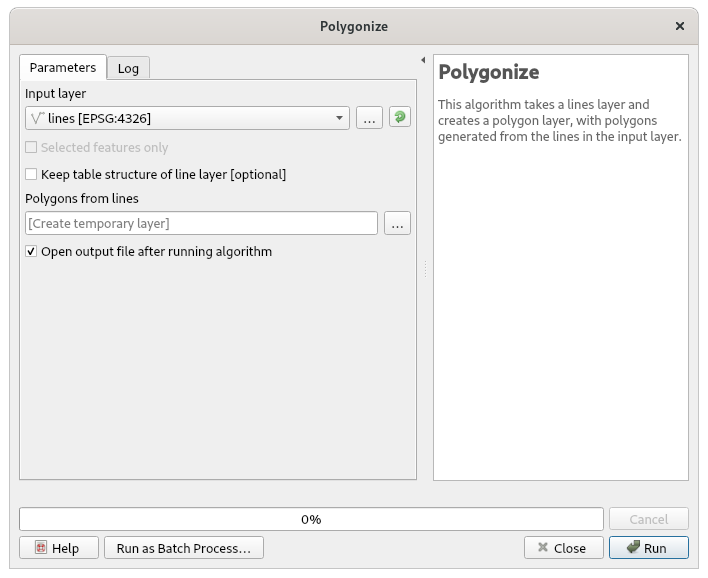
\includegraphics[width=10cm]{./pictures/5.1/polygonize.png}
  \caption{Rozhraní nástroje Polygonize v softwaru QGIS Desktop.}
  \label{fig:polygonize}
\end{figure}

\section{PostGIS}
	Obdobně byl testován i nástroj PostGIS. Zde už se nejedná o desktopovou aplikaci, jako tomu bylo u výše testovaných softwarů. PostGIS je nadstavba pro objektově-relační databázi PostgreSQL. Jedná se tedy o rozšíření databáze o podporu geo\-grafických objektů a funkcí. Je často využíván k uchování geografických dat a analýz nad nimi. Nutno podotknout, že PostGIS využívá pro většinu svých o\-pe\-ra\-cí taktéž knihovnu \textit{GEOS} psanou v programovacím jazyce \textit{C++}, kterou následně poskytuje uživateli přes standardní dotazovací jazyk SQL.
	
	Postup polygonizace zde bude o něco složitější. Budeme nuceni polygonizaci rozdělit do dvou kroků, jak bylo řečeno v kapitole~\ref{chap:reserzepouzivanychalgoritmu}. Nejprve se tedy zaměříme na doplnění průsečíků linií a poté provedeme vlastní polygonizaci. Pro doplnění průsečíku linií nám PostGIS nabízí hned dvě možnosti.
	
\subsubsection{Funkce \textit{ST\_UnaryUnion}}
	První z možností je využít funkci \textit{ST\_UnaryUnion}. Tato funkce rozpouští linie tak, že sdílí maximálně koncový bod s jinými liniemi. Tímto způsobem můžeme připravit podkladové linie pro následnou polygonizaci. Nevýhoda této funkce je ovšem v její časové složitosti. Oproti druhé možnosti, tedy funkci \textit{ST\_Node}, dosahuje značně vyšších časů pro výpočet~\citep{PostGIS_software}.
	% select st_unaryunion(st_collect(st_linemerge(geom))) from spageti_small;
	
\subsubsection{Funkce \textit{ST\_Node}}
	Druhá možnost a alternativa funkce \textit{ST\_UnaryUnion} je funkce \textit{ST\_Node}. Tato funkce taktéž rozpojuje linie v průsečících. Nicméně oproti předchozí zmíněné pracuje v mnohem kratších časech. Výhodou obou těchto funkcí může být možnost pracovat s 3D daty~\cite{PostGIS_software}.

% https://trac.osgeo.org/geos/ticket/962

\subsubsection{Funkce \textit{ST\_Polygonize}}
	Pokud máme průsečíky doplněny, můžeme přistoupit k vlastní tvorbě polygonů. K tomu nám poslouží funkce \textit{ST\_Polygonize} využívající metod knihovny GEOS. Výstupem této funkce je pak geometrická kolekce obsahující polygony~\cite{PostGIS_software}.

\begin{figure}
\begin{minted}
{postgresql}
SELECT st_polygonize(lines_nodded.geom) AS geom
FROM (
        SELECT st_node(st_collect(st_linemerge(geom))) AS geom
        FROM lines_small
    ) AS lines_nodded
\end{minted}
\caption{Příklad tvorby polygonů v PostGIS.}
\label{fig:SQL_polygonize}
\end{figure}


	
	
	
	
\chapter{Implementace algoritmu do GeoTools}
	Pro implementaci polygonizačního algoritmu byla vybrána open-source knihovna pro programovací jazyk java \textit{GeoTools}. V současné době je \textit{GeoTools} součástí \textit{OSGeo}, což je nezisková organizace, snažící se podporovat open-source geoprostorové technologie. Mimo \textit{GeoTools} organizace zastupuje řadu dalších projektů, mezi které patří v desktopových aplikacích textit{QGIS}, \textit{GRASS GIS}, mezi mapové servery \textit{MapServer}, \textit{GeoServer} a mezi knihovnami jsou nejvýznamějšími zástupci \textit{GEOS}, \textit{GDAL}, \textit{PROJ}, nebo \textit{JTS}. Právě zmíněná knihovna \textit{JTS} tvoří základní kámen pro \textit{GeoTools}, jelikož jsou v ní definovány základní geometrické tipy a operace pro práci s prostorovými daty. Možná více známá knihovna než \textit{JTS} je knihovna \textit{GEOS}, což není nic jiného než přepis knihovny z javy do C++.
	
	
\
	
	
	jako je například \textit{QGIS}, \textit{GRASS GIS}, \textit{MapServer},

	


\chapter{Implementace algoritmu do GeoTools}
\label{chap:implementacealgoritmudogeotools}
	Pro implementaci polygonizačního algoritmu byla vybrána open-source knihovna pro programovací jazyk Java \textit{GeoTools}. V současné době je \textit{GeoTools} součástí \textit{OSGeo}, což je nezisková organizace, podporující open-source geoprostorové technologie. Mimo \textit{GeoTools} organizace zastupuje řadu dalších projektů, mezi které patří v desktopových aplikacích textit{QGIS}, \textit{GRASS GIS}, mezi mapové servery \textit{MapServer}, \textit{GeoServer} a mezi knihovnami jsou nejvýznamějšími zástupci \textit{GEOS}, \textit{GDAL}, \textit{PROJ}, nebo \textit{JTS}. Právě zmíněná knihovna \textit{JTS} tvoří základní kámen pro \textit{GeoTools}, jelikož jsou v ní definovány základní geometrické typy a operace pro práci s prostorovými daty. Možná více známá knihovna než \textit{JTS} je knihovna \textit{GEOS}, což je přepis knihovny z Javy do C++. \cite{OSGeo} \cite{GeoTools}
	
\section{GeoTools plug-in systém}
	Většina \textit{open-source} projektů je založena na příspěvcích od komunity vývojářu. Proto jsou projekty vytvořeny tak aby byli snadno rozšiřitelné o nějakou funkcionalitu. Výjimkou není ani projekt \textit{GeoTools}. Snaha vývojářů je tedy taková, co nejvíce usnadnit tvorbu zásuvných modulů. Na webových stránkách \textit{GeoTools}\cite{GeoTools} najdeme velmi podrobný tutoriál pro implementaci uživatelských funkcí a jiných dalších komponent. K tomuto účelu je využíváno technologie Java Service Provider Interface.
	
\subsection{Java Service Provider Interface}
	Java SPI přišla s nástupem Javy 6, která byla představena v roce 2006. Tato technologie umožňuje vyhledat a načíst implementaci daného rozhraní a tak dodat funkčnost. Této metody je využíváno například u přístupu k databázím pomocí JDBC, kdy třetí strana má možnost implementovat ovladače pro jakoukoli databázi a tak rozšířit funkčnost JDBC. Základními prvky SPI jsou:
	
\begin{itemize}
	\item Service
	\item Service provider interface
	\item Service provider
\end{itemize}	
	
\subsubsection{Service}
	Též hojně označované jako \textit{služba}. Jedná se o API se kterým programátor pracuje, aniž by věděl že 


\subsubsection{Service provider interface}
	Také nazývané \textit{rozhraní poskytovatele služeb}. Je rozhraní nebo abstraktní třída, která slouží jako koncový bod služby. Toto rozhraní nebo abstraktní třída je dále implementována poskytovatelem služeb.
	
	
\subsubsection{Service provider}
	V Češtině se někdy používá označení \textit{poskytovatel služeb} nebo zkráceně jen \textit{poskytovatel}. Jedná se o implementaci \textit{rozhraní poskytovatele služeb}. V analogii na \textit{JDBC} se může jednat o implementaci do konkrétní databáze.


\subsubsection{ServiceLoader class}




\subsection{Návrhový vzor Factory}



\subsection{První implementace}

	


\chapter{Závěr}
\label{chap:zaver}

		V této práci byla zpracována stručná rešerše literatury, zabývající se metodami odstranění zkreslení z fotografických snímků. Vybrané metody odstranění zkreslení jsou dále v práci popsány. Jako nejvhodnější způsob se jevilo odstranění zkreslení za pomoci \textit{Brownova} distorzního modelu, který je v obdobných softwarech často používaný.
	
	Hlavním cílem této práce bylo vytvořit softwarové řešení tohoto problému, které bude mít moderní grafické rozhraní. Pro tvorbu softwaru byl zvolen programovací jazyk \textit{C++} s využitím knihoven \textit{Qt}. Tento nástroj usnadnil tvorbu grafického rozhraní, které je zkoncipováno tak, aby mohl uživatel intuitivně program ovládat a nebylo zapotřebí podrobnější znalosti softwaru. Program byl sestaven pro platformu \textit{Windows}, jelikož je však jazyk \textit{C++} s knihovnami \textit{Qt} určen pro různé platformy, nic nebrání tento program sestavit i pro \textit{Linux} či \textit{macOS}, což tento software dělá použitelnější pro větší okruh lidí. Dalším vylepšením vytvořeného programu \textit{DistortionRemover} by do budoucna mohlo být obohacení o výpočet parametrů prvků vnitřní orientace kamery, které v současné době musí uživatel získat z jiného softwaru, či jiného zdroje. Velkým zlepšením by mohlo také být práce s obrazovými daty typu RAW, zamezilo by se tak velkým ztrátám kvality při opravě snímku. Samozřejmostí je opravení chyb, v programu, které budou odhaleny rozsáhlejším používáním. 
		
	Ve finální části, je předvedena práce s programem na příkladu historického stavebního objektu z databáze PhotoPa a jsou nastíněny další možné postupy zpracování.

	




% Vysázení seznamu zkratek

\begin{seznamzkratek}{ABCDE}

	\novazkratka{GIS}
	      {GIS}
	      {Geografický informační systém}

      \novazkratka{OSGeo}
	      {OSGeo}
	      {Open Source Geospatial Foundation}
      
      \novazkratka{GEOS}
	      {GEOS}
	      {Geometry Engine, Open Source}
	      
	  \novazkratka{OGC}
	      {OGC}
	      {Open Geospatial Consortium}
	      
	      
	      
	  \novazkratka{GPL}	
	      {GPL}
	      {Všeobecná veřejná licence (General Public License)}
	      
	  \novazkratka{LGPL}	
	      {LGPL}
	      {Lesser General Public License}
	      
	   \novazkratka{SPI}	
	      {SPI}
	      {Java Service Provider Interface}
	      
	   \novazkratka{JDBC}	
	      {JDBC}
	      {Java Database Connectivity}
	      
	   \novazkratka{API}	
	      {API}
	      {Aplication Interface}
	      
	   \novazkratka{RGB}	
	      {RGB}
	      {Barevný model Red, Green, Blue}

	   \novazkratka{GDF/DIME}	
	      {GDF/DIME}
	      {Geographic Base File/Dual Independent Map Encoding}
	      
	      

\end{seznamzkratek}

% Vysázení seznamu obrázků
\seznamobrazku/obrazky

% Literatura
\nocite{*}
\def\refname{Literatura}
\bibliographystyle{mystyle}
\bibliography{literatura}

%% Začátek příloh
\def\figurename{Figure}%
\prilohy
%
%% Vysázení seznamu příloh
%\seznampriloh
%
%% Vložení souboru s přílohami
%%%%%%%%%%%%%%%%%%%%%%%%%%%%%%%%%%%%%%%%%%%%%%%%%%%%%%%%%%%%%%%%%%%%%%%%%%%%%%%%%%%
%%                 PŘÍLOHA - UŽIVATELSKÁ PŘÍRUČKA                                %%
%%%%%%%%%%%%%%%%%%%%%%%%%%%%%%%%%%%%%%%%%%%%%%%%%%%%%%%%%%%%%%%%%%%%%%%%%%%%%%%%%%%
\chapter{Srovnání polygonizace v ArcGIS Desktop a QGIS Desktop}
\label{chap:srovnani}
Srovnání bylo provedeno na testovacích datech, které poskytl \textit{Ing. Jan Růžička, Ph.D.}. Jelikož nemohla být poskytnuta reálná data, jedná se o uměle vygenerované linie, které jsou dle slov doktora Růžičky obdobného charakteru a velikosti. Data obsahují celkem 10000 linií. Tato data byla dále testována ve zmenšené formě a to s 1000 a 100 liniemi.

\section{Parametry počítače}
\begin{itemize}
\item \textbf{Operační systém:} 
\item \textbf{Procesor:} 
\item \textbf{RAM:} 
\end{itemize}

\section{ArcGIS Desktop}

\section{QGIS Desktop}


\chapter{Elektornické přílohy}
\label{user-guide}

\section{CD disk}

\pagenumbering{Roman}
\label{app:cd}
    
    \begin{description}
        \item[\tt BP-DistortionRemover.pdf] ~ \\ text bakalářské práce ve formátu *.pdf,
    	
        
        \item[\tt DistortionRemover/] ~ \\ adresář s programem,
        \begin{description}
        		
        		\item[\tt DistortionRemover.exe] ~ \\ Spustitelný soubor aplikace,
        		
        		\item[\tt License.txt] ~ \\ textový soubor s popisem licence,
        		
            	\item[\tt Source/] ~ \\ adresář obsahující zdrojové kódy,
            	\begin{description}
            			\item[\tt DistortionRemover.pro] ~ \\ projektový soubor,
            			\item[\tt main.cpp] ~ \\ zdrojový kód funkce main,
            			\item[\tt distortionremover.h] ~ \\ hlavičkový soubor distortionremover,
            			\item[\tt distortionremover.cpp] ~ \\ zdrojový soubor distortionremover obsahující funkce pro chod programu,
            			\item[\tt ui\_distortionremover.h] ~ \\ hlavičkový soubor grafického rozhraní,
            			\item[\tt distortionremover.ui] ~ \\ soubor obsahující grafické prostředí v XML,
            			\item[\tt picturetransformation.h] ~ \\ hlavičkový soubor picturetransformation,
            			\item[\tt picturetransformation.cpp] ~ \\ zdrojový soubor picturetransformation obsahující výpočetní funkce,
            			\item[\tt resource.qrc] ~ \\ soubor pro uložení binárních souborů do aplikace který obsahuje ikonu,
            			\item[\tt DR.ico] ~ \\ ikona programu.

            	\end{description}
        \end{description}
    \end{description}



% Konec dokumentu
\end{document}

